%\documentclass[10pt]{article}
%\usepackage[usenames]{color} %usato per il colore
%\usepackage{amssymb} %maths
%\usepackage{amsmath} %maths
%\usepackage[utf8]{inputenc} %utile per scrivere direttamente in caratteri accentuati
%\begin{document}
\label{MEsection}
The event-mixing technique is used for correcting the raw correlation distribution for effects arising
from the detector limited acceptance in rapidity and detector spatial inhomogeneities. The calculation of the Event
Mixing correlation distribution is performed online. %, following the strategy and the code developed for the \textit{PWGCF} correlation analyses.
An event pool is created, where events preceding the one containing a D candidate are stored based on their properties (position of the vertex along the z axis and multiplicity).
Each time a D meson candidate is found in an event, only the events contained in the same pool as the event under analysis is used to evaluate the correlations for the event mixing correction.% the correlation analysis on the mixed events is performed if the pool satisfies the conditions defined at its creation, being the same as described for the pp analysis (As well as the conditions for refreshing the pools).

For $\Dzero$ and $\Dplus$, an offline approach for the mixed-event correction has been developed. In this approach, D-meson triggers and associated tracks from every analyzed event are stored in dedicated TTree, together with the needed kinematic information to build correlation distributions, and with identifiers of the events to which they belong. In this way, it is possible to correlate each D meson with all the tracks belonging to the same pool over the full event sample, and not being limited to the same subjob as for the online analysis. This allows to increase the statistics of the mixed-event correlation distributions. If was verified that online and offline approaches are fully compatible within the statistical uncertainties.

The multiplicity and z vertex position bins for the pools used in the p-Pb analysis (for both approaches) are the following:
\begin{itemize}
\item Multiplicity bins: $\left(0,40\right);\left(40,65\right);\left(65,+\infty\right)$ (THESE ARE BEING SLIGHTLY CHANGED)
\item Vertex z $(cm)$ = $\left(-10,-2.5\right);\left(-2.5,2.5\right);\left(2.5,10\right)$ (THESE ARE BEING SLIGHTLY CHANGED)
\end{itemize}
%(\ref{tab:em})

In an ideal case, the mixed event distribution is expected to have a constant flat distribution as function of $\Delta\phi$ and a triangular shaped distribution in $\Delta\eta$
deriving from the limited $\eta$ acceptance of the detector. In case, instead of detector inefficient regions, or holes, in the same angular position for D meson and associated tracks, these structures produce an excess of correlations at $\Delta\phi=0$ in the $\Delta\phi$ distribution. The obtained distribution is used as a weight in each correlation bin, i.e, the corrected correlation distribution is calculated as follows:
\begin{equation}
\label{eq:mixing}
\frac{dN^{corr}\left(\Delta\phi \Delta\eta\right)}{d\Delta\phi d\Delta\eta} = \frac{\frac{dN^{SE}\left(\Delta\phi \Delta\eta\right)}{d\Delta\phi d\Delta\eta} }{\frac{dN^{ME}\left(\Delta\phi \Delta\eta\right)}{d\Delta\phi d\Delta\eta} }\frac{dN^{ME}\left(0,  0\right)}{d\Delta\phi d\Delta\eta}
\end{equation}
In the previous equation, the last term stands for the average of the bins in the region $-0.2 < \Delta\eta < 0.2$, $-0.2 < \Delta\phi < 0.2$ (multiple bins are used to minimize the effect of statistical fluctuations on the normalization of the mixed-event plots).
This kind of normalization, adopted in the analysis of hadron-hadron correlations, relies on the fact that at $(\Delta\eta,\Delta\phi)=(0,0)$ the trigger and associated particle experience the same detector effects. In the D meson case this is true only on average and not at very low $\pt$, since D mesons are reconstructed from particles that can go
in different detector region. However, $(\Delta\eta,\Delta\phi)=(0,0)$ is in any case
the region with maximum efficiency for the pairs (both correlated and uncorrelated). Thus the same convention was adopted.

The mixed-event correlation distributions are built in both D meson signal and sideband regions. Both are
corrected with the relative distributions. An example of the mixed-event distributions, and of the outcome of the mixed-event correction, is provided in Figures \ref{fig:DzeroME} and \ref{fig:Dsubtr2D}. The expected triangular shape in $\Delta\eta$, for the mixed-event distributions, addresses the effect of the limited detector pseudo-rapidity acceptance. Note that the mixed-event distribution is limited to the interval $\left|\Delta\eta\right|<1$: the decision to limit the mixed-event correction, and thus the whole analysis, to this range was taken in order to avoid the so-called ``wing effect", i.e. the wing-like structures arising in the correlation distribution at large $\Delta\eta$ due to the
limited filling of the correlation bins in that region.

\begin{figure}
\centering
{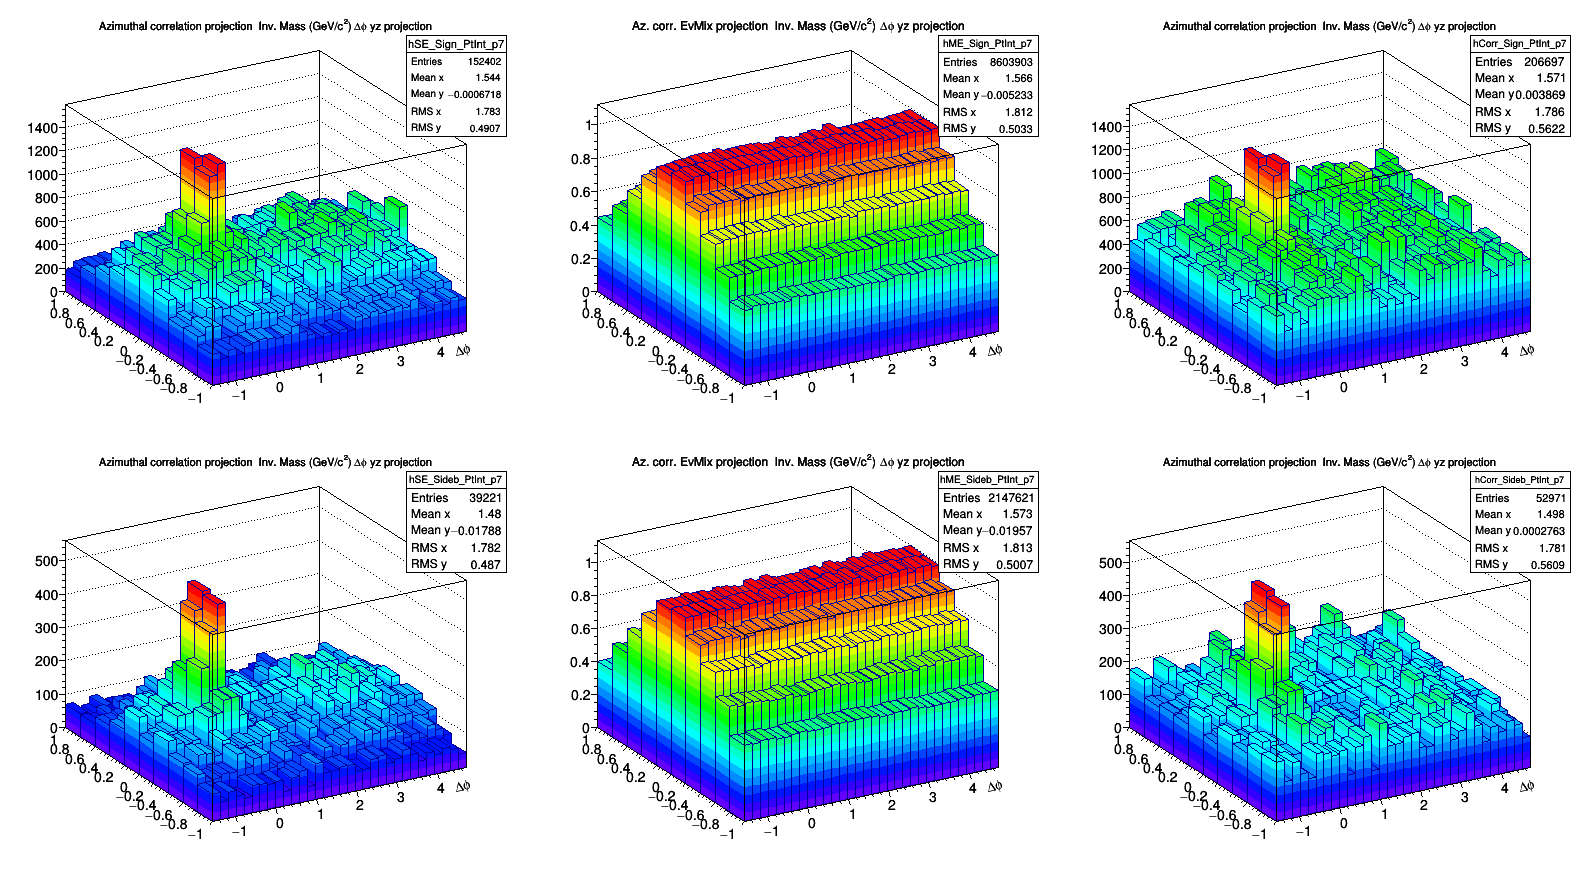
\includegraphics[width=1\linewidth]{figures/Dzero/CorrSEandME_Dzero_Canvas_PtIntBins9to11_pool7_thr0dot3to99dot0.png}}

 \caption{$\Dzero$ meson ($\Delta\phi$,$ \Delta\eta$) correlation for in the signal region (top row) and sidebands (bottom row) from  Single Event (left) and Mixed Event analysis (center) for high $p_\mathrm{T}$: $8 < p_\mathrm{T}<16$ GeV/c with associated $p_\mathrm{T}$ > 0.3 GeV/c. The right column shows the SE/ME corrected distributions.}
\label{fig:DzeroME}
\end{figure}

\begin{figure}
\centering
{\includegraphics[width=0.9\linewidth, height = 7cm]{figures/Dzero/h2D_Dzero_Subtr_Canvas_PtIntBins4to5_PoolInt_thrdot3to99dot.png}}
{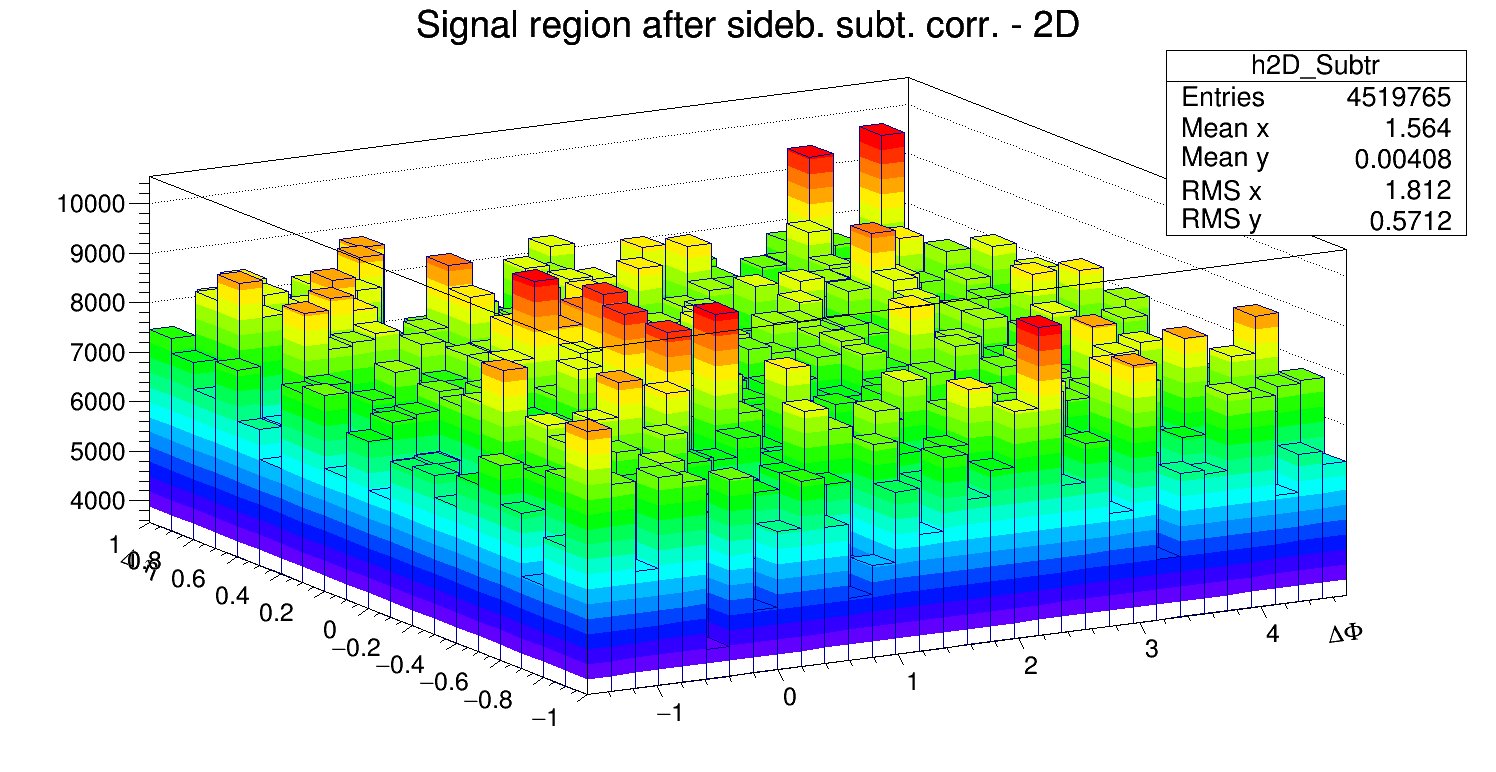
\includegraphics[width=0.9\linewidth, height = 7cm]{figures/Dstar_wEFF/h2D_Dstar_Subtr_Canvas_PtIntBins2to3_PoolInt_thr0dot3to99dot0.png}}
{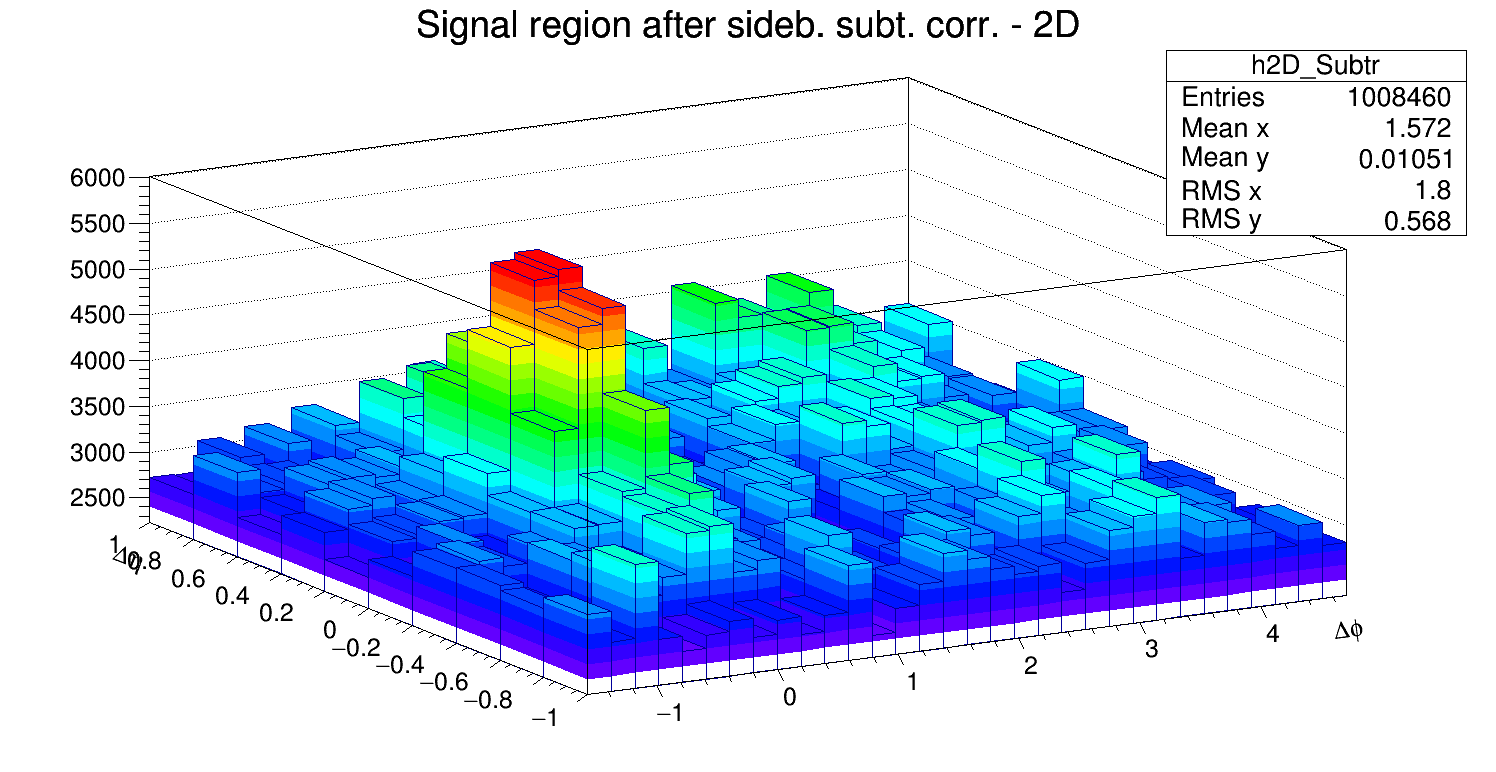
\includegraphics[width=0.9\linewidth, height = 7cm]{figures/DplusPlotsweff/h2D_Dplus_Subtr_Canvas_PtIntBins8to10_PoolInt_thr0dot3to99dot0.png}}
\caption{Top: ($\Delta\phi$, $\Delta\eta$) correlation distribution of $D^{0}$-h with $3 < \pt < 5$ GeV/c and associated track kinematic range: $0.3 < \pt < 1.0$ GeV/c
Mid: ($\Delta\phi$, $\Delta\eta$) correlation distribution of $D^{*+}$-h with $3 < \pt < 5$ GeV/c and associated track $\pt$ Threshold: $\pt > 0.3$ GeV/c
Bottom: ($\Delta\phi$, $\Delta\eta$) correlation distribution of $D^{+}$-h with $8 < \pt < 16$ GeV/c and associated track $\pt$ threshold: $\pt > 0.3$ GeV/c. All the plots are shown after the mixed-event correction and the sideband subtraction.}
\label{Dsubtr2D}

\end{figure}
\clearpage
%\end{document}
